\begin{frame}{Modelo SIRS}
    O modelo SIRS divide a população em indivíduos suscetíveis ($S$) à doença, infectados ($I$) e recuperados ($R$).
    
    Uma parte da população de suscetíveis pode se infectar (termo $\beta.S.I$). Os indivíduos infectados podem se recuperar com uma determinada probabilidade (termo $\alpha.I$) e os indivíduos recuperados podem voltar a ser suscetíveis à doença (termo $\gamma.R$). 
    
    \begin{equation}\label{eq:sirs}
        \begin{array}{lr}
        \frac{dS}{dt} = -\beta.S.I + \gamma.R
        \\
        \\
        \frac{dI}{dt} = \beta.S.I - \alpha.I
        \\
        \\ 
        \frac{dR}{dt} = \alpha.I - \gamma.R
        \end{array}
    \end{equation}
\end{frame}

\begin{frame}{Modelo SIRS - Representação no Software}
    \begin{figure}
        \centering
        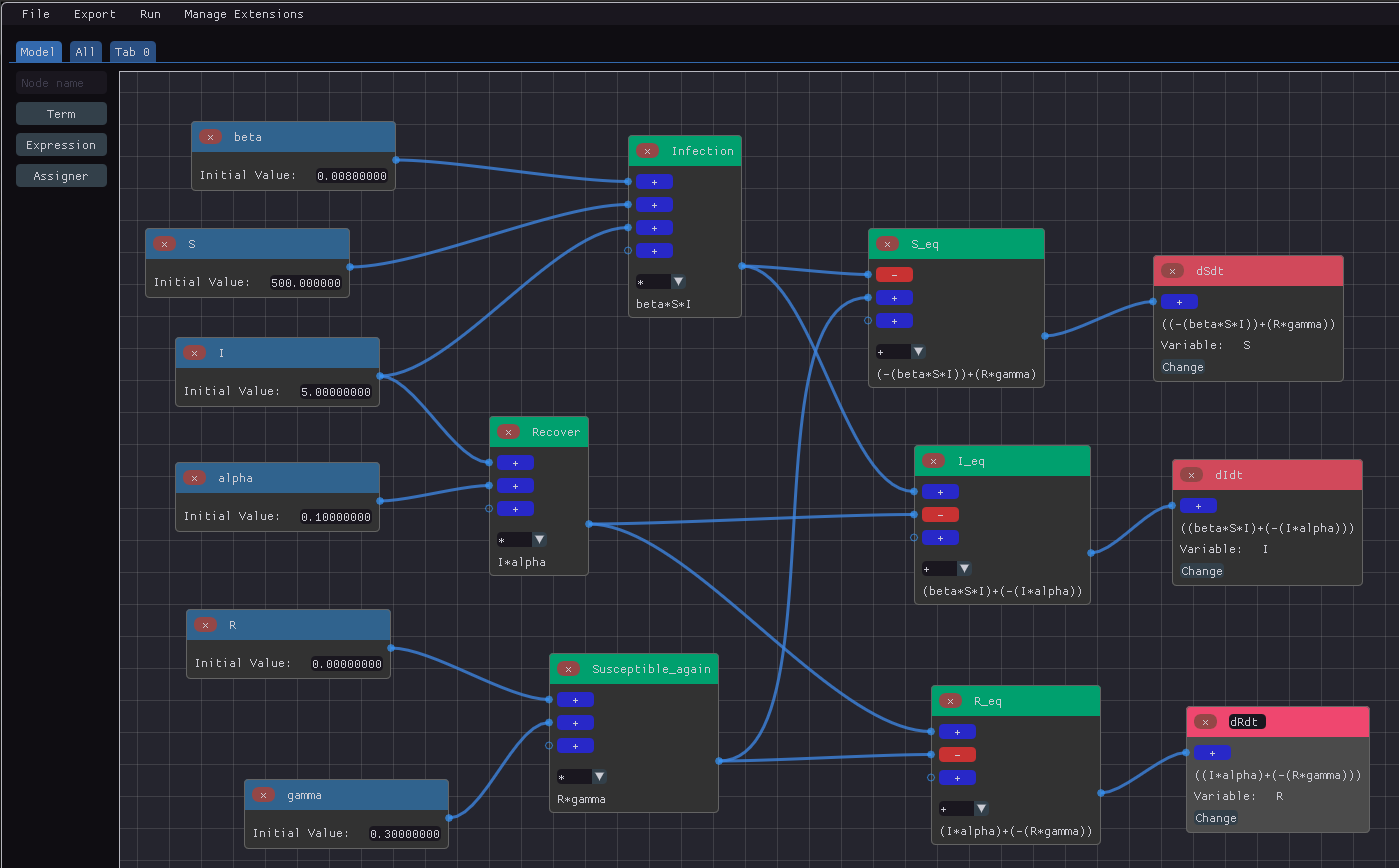
\includegraphics[height=\textheight]{contents/imgs/modelos/sirs.png}
    \end{figure}
\end{frame}

\begin{frame}{Modelo SIRS - Resultados}
    \begin{columns}
        \begin{column}{.2\textwidth}
            \[
            \begin{array}{llr}
                S_0 & = & 500\\
                I_0 & = & 5\\
                R_0 & = & 0\\
                \alpha & = & 0.1\\
                \beta & = & 0.008\\
                \gamma & = & 0.3\\
                \end{array}
            \]
        \end{column}
        \begin{column}{.8\textwidth}
            \begin{figure}
                \centering
                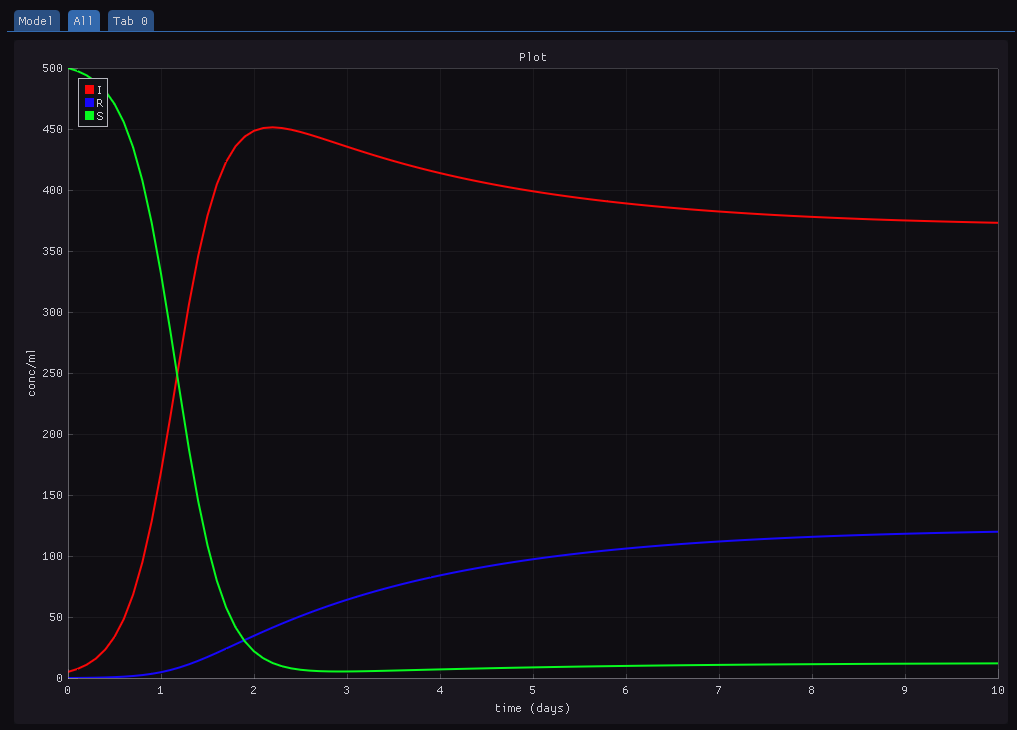
\includegraphics[height=\textheight]{contents/imgs/modelos/resultado-sirs.png}
            \end{figure}
        \end{column}
    \end{columns}
\end{frame}